\newpage

\section{marche aléatoire}

\begin{figure}[h]
    \centering
    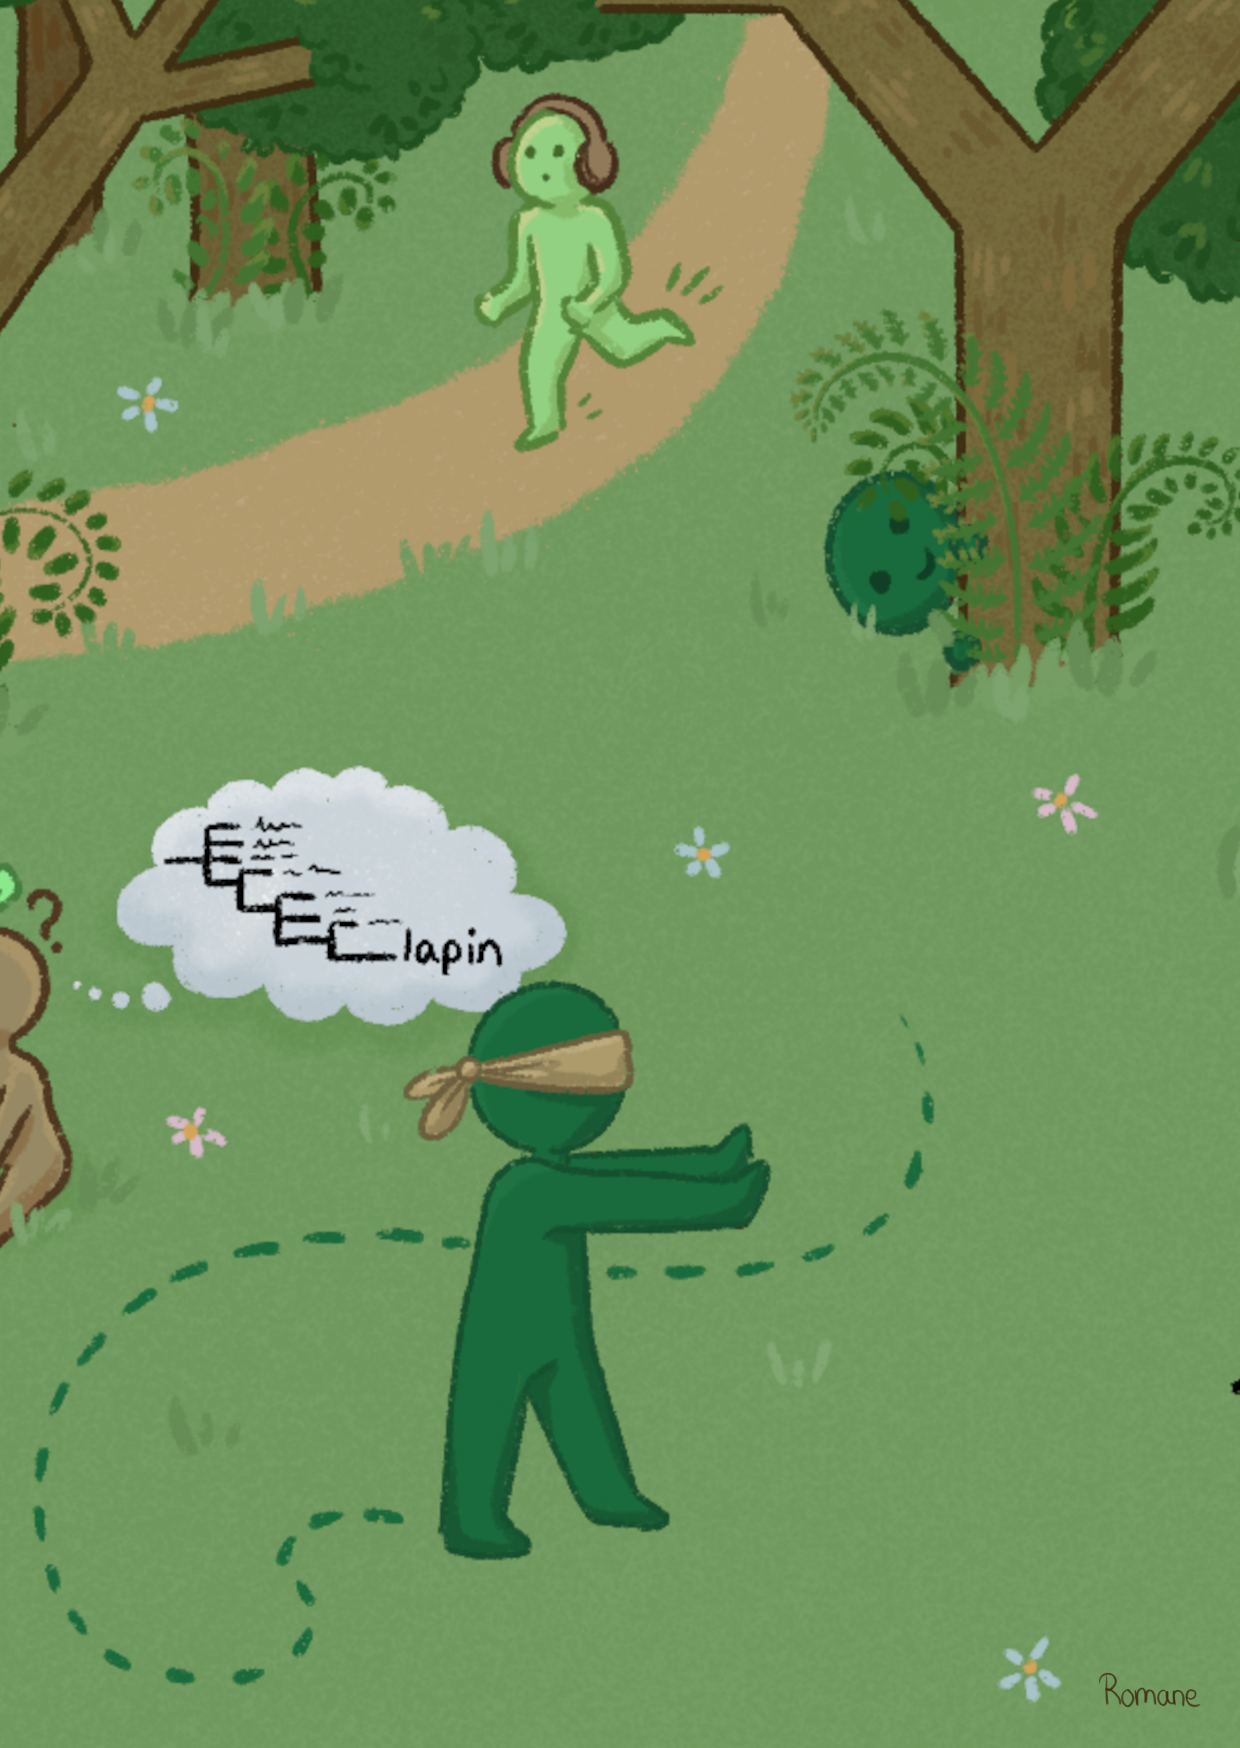
\includegraphics[height=0.5\textheight]{Cartes_postales/carte10-marche.png}\label{fig:c10}
    \caption{Carte postale: marche}
\end{figure}

Imaginons que tu te retrouves au milieu des rues de Manhattan, à New York, et tu commences à marcher. A chaque intersection, tu choisis aléatoirement la direction que tu prends. Si tu continues ce processus indéfiniment, tu finiras toujours par revenir à ton point de départ. Et ce, même s'il y avait une infinité de rues. Les probabilités permettent de trouver de l'ordre dans le chaos en établissant des lois universelles sur des comportements imprévisibles.
\medskip

C'est un concept très utile pour modéliser le hasard au quotidien, comme la trajectoire des molécules d'un parfum qui se diffuse dans une pièce ou les fluctuations de la bourse. En pratique, le monde réel complexifie les calculs (interactions physiques, crises financières), ce qui pousse les mathématiciens à chercher des modèles toujours plus précis. En couplant ces théories à des données de qualité, on réussit à prédire l'imprévisible grâce à des intervalles de confiance. \\


